\documentclass[12pt,a4paper]{article}
\usepackage[utf8]{inputenc}
\usepackage[frenchb]{babel}
\usepackage[T1]{fontenc}
\usepackage{amsmath}
\usepackage{amsfonts}
\usepackage{amssymb}
\usepackage{graphicx}
\usepackage[left=1cm,right=1cm,top=2cm,bottom=2cm]{geometry}
\begin{document}
\textbf{Analyse de réponses temporelles de systèmes asservis}

Des essais d'un système asservi en position ont été réalisés pour différents réglages d'un correcteur et des mesures ont été faites qui permettent de valider certains réglages selon les exigences du cahier des charges. 


\begin{center}
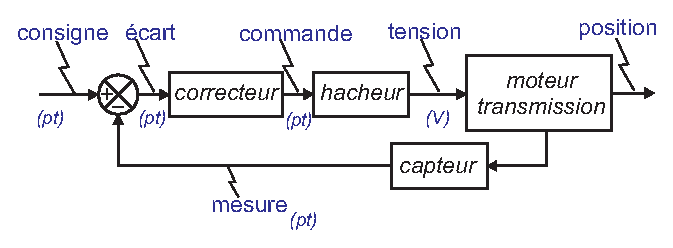
\includegraphics[scale=1]{images/schema-bloc.eps} 
\end{center}

Les courbes construites à partir de huit parmi de très nombreux essais sont données en annexe; il est possible de déterminer deux grandeurs intéressantes:
\begin{itemize}
\item l'erreur statique de position : c'est la valeur vers laquelle tend  l'écart  consigne - mesure si la position se stabilise; c'est le cas pour les essais à étudier.
\item le temps de réponse à \textbf{5\%} qui correspond à la date à partir de laquelle le signal de mesure reste à l'intérieur d'une bande de \textbf{+/-5\%} par rapport à l'asymptote du signal de mesure.
\end{itemize}

\begin{center}
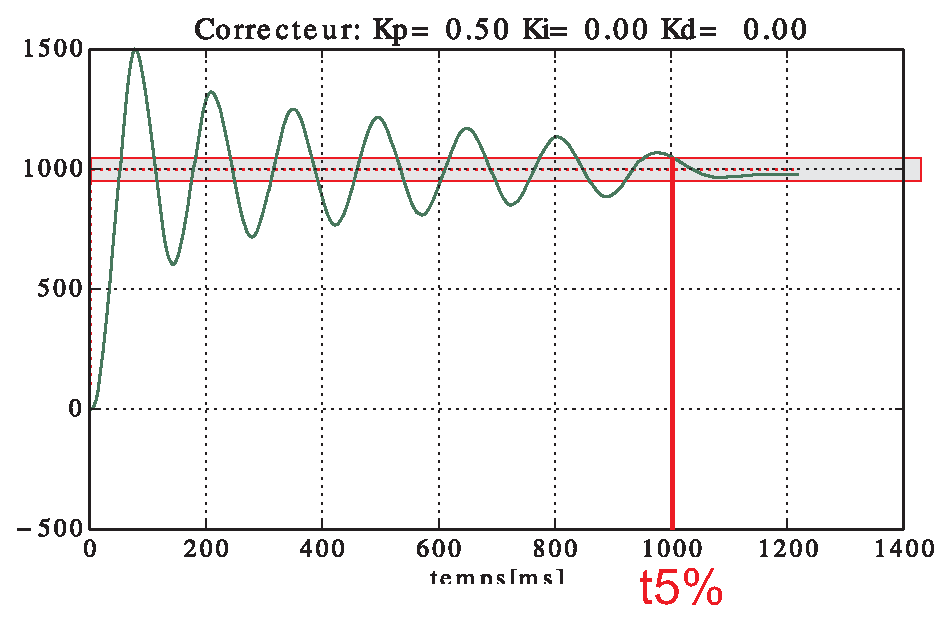
\includegraphics[scale=0.8]{images/t5-dessin.eps} 
\end{center}

Le système de commande du processus est numérique, la commande est élaborée avec une période très proche de \textbf{3}ms, les mesures sont effectuées au même rythme. 

Les résultats sont fournis sous la forme de fichiers csv avec une en-tête dans laquelle la première ligne sera indiquée sur le tracés car elle contient des données de réglages, suivent 3 autres non utiles.
Le fichier continue par les données selon trois colonnes:
\begin{itemize}
\item le temps en milliseconde
\item la consigne en point 
\item la mesure en point
\item la commande en point
\end{itemize}

\medskip

\textbf{Exemple de début de fichier à traiter:}

\hspace{3cm}\begin{minipage}[c]{0.5\linewidth}
\begin{verbatim}
Correcteur: Kp= 0.10 Ki= 0.00 Kd=  0.00
 Consigne [pt] : 1000.00
date;Consigne;Mesure;Commande
[ms];[pt];[pt];[pt]
0; 0; 0; 0
1; 1000; 0; 100
4; 1000; 1; 99
7; 1000; 4; 99
10; 1000; 13; 98
13; 1000; 22; 97
16; 1000; 35; 96
19; 1000; 51; 94
22; 1000; 70; 93
25; 1000; 93; 90
28; 1000; 122; 87
\end{verbatim}
\end{minipage}

\medskip

Les fichiers à traiter correspondent à des réponses d'un système avec réglage assurant la stabilité et on est assuré que les 20 dernières lignes de données correspondent à l'état stabilisé.
\bigskip

\textbf{Objectif:} élaborer un programme en Python qui réalise:
\begin{itemize}
\item la lecture du fichier avec extraction du texte de la première ligne
\item la détermination de la valeur moyenne des 20 dernières lignes de la position et l'erreur statique de position en valeur relative
\item la détermination du temps de réponse à 5\% .
\item le tracé de la courbe de mesure en fonction du temps avec:
\begin{itemize}
\item en titre la première ligne du fichier
\item l'asymptote de la mesure
\item les deux horizontales délimitant la bande de 5\% 
\item le tracé de la consigne en pointillé.
\end{itemize}
\end{itemize}  

\medskip

\textbf{Données:}
dans un dossier TP9-Complement: un fichier TP8-Complement.py, ébauche du travail et un sous-dossier data qui contient 8 fichiers de données à traiter.

  
\end{document}